\subsection{Rede neural artificial}

Uma rede neural artificial é uma representação matemática de unidades de processamento conectadas chamadas de neurônios artificiais. Essa arquitetura simula sinapses, cada sinal trocado entre os neurônios pode aumentar ou atenuar os sinais de outros durante o aprendizado\cite{ml_and_dp}.
\begin{figure}[H]
	\centering
	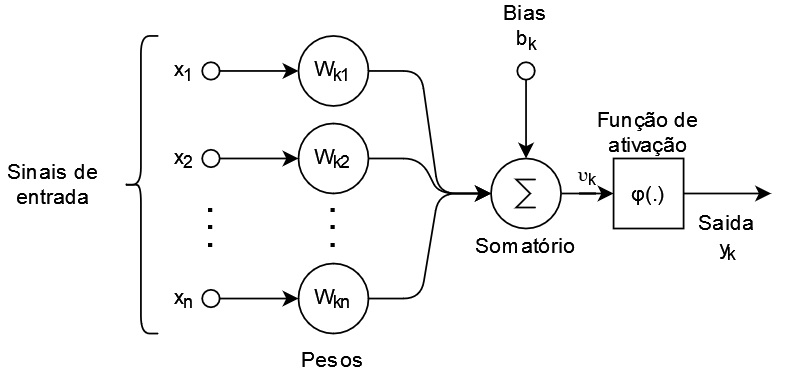
\includegraphics[width=0.8\textwidth]{figures/neuronio.png}
	\caption{Modelo de um neurônio não-linear \cite{haykin1999neural}.}
	\label{fig:neuronio}
\end{figure}

Observando a figura \ref{fig:neuronio} é possível observar o funcionamento de um neurônio $k$. Os sinais de entradas são partes de um vetor $x$ de tamanho $n$, sendo o vetor composto por $x_1, x_2 ... x_n$. Essas componentes são combinadas em uma soma ponderada utilizando seus respectivos pesos, $w_{k1}, w_{k2}...w_{kn}$, formando assim a seguinte equação  \apud{marti2017aprendizado}{haykin1999neural}:

\begin{equation}
	\upsilon_k = \sum_{i=1}^n (x_i * w_{ki})
\end{equation}

O resultado dessa equação produz o potencial de ativação $\upsilon_k$, esse resultado é somado com o \textit{bias} ou viés $b_k$ para manipular a saída $y_k$ do neurônio, essa soma é posta em uma função não-linear nomeada de função de ativação $\varphi(.)$, essas funções mapeiam a saída em um intervalo $[0, 1]$ ou $[1, -1]$. A função de saída pode ser representada com a seguinte equação \apud{marti2017aprendizado}{haykin1999neural}:

\begin{equation}
	y_k = \varphi(\upsilon_k + b_k)
\end{equation}

O aprendizado ocorre na fase de treinamento onde é ajustando os pesos $w_k$ e o viés $b_k$ de cada neurônio $k$. Os pesos $w_k$ são utilizados para calcular a taxa de crescimento da função e o viés $b_k$ é necessário para descolar a saída da função. Com isso é possível modelar uma função linear $y=w^T*x+b$ \cite{marti2017aprendizado}.

Para cada amostra o modelo compara os resultados dos valores atuais dos pesos $w_k$ e viés $b_k$ com o resultado esperado (alvo). Uma função de perda é utilizada para gerar um vetor de gradientes e para quantificar o erro encontrado para a configuração atual do modelo. O modelo atualiza os pesos $w_k$ e os viés $b_k$ no sentido contrário do vetor de gradientes, buscando minimizar a função de custo de acordo com uma taxa de aprendizado(\textit{learning rate}), esse processo é chamado de retropropagação — ou backpropagation — que será explicado melhor posteriormente \cite{marti2017aprendizado}.

Ao combinar diversos neurônios artificiais forma-se uma rede neural artificial. Essas redes buscam simular o processamento de informação do cérebro humano \cite{ferneda2006redes}.
Nas redes neurais os neurônios são organizados em grupos de unidade de processamento chamados camadas. A primeira e a última camada são nomeadas de camada de entrada e camada de saída e as demais de camadas ocultas. As camadas mais próximas da entrada são responsáveis por identificar características mais primitivas e as seguintes combinam essas informações para identificar padrões mais complexos \cite{marti2017aprendizado}.

Nas redes neurais os neurônios são organizados em grupos de unidade de processamento chamados camadas. A primeira e a última camada são nomeadas de camada de entrada e camada de saída e as demais de camadas ocultas. As camadas mais próximas da entrada são responsáveis por identificar características mais primitivas e as seguintes combinam essas informações para identificar padrões mais complexos \cite{marti2017aprendizado}.
